\documentclass[journal]{IEEEtran}

\usepackage{cite}
\usepackage{graphicx}
\usepackage{url}
\usepackage[hidelinks]{hyperref}

\begin{document}

\title{Assessing How External Data Address Information Gaps in
Montandon-Based Disaster Preparedness Question Answering}

\author{Jeongmin An, Jehan Bugli, and Aidan Carlisle}

\maketitle

\begin{abstract}
Disaster preparedness and the development of Early Action Protocols
(EAPs) require evidence about past hazards, impacts, response activities,
and financing. This evidence is distributed across structured disaster
records, news reports, weather observations, and spatial data. We
investigate which information needs remain unanswered in
Montandon-based disaster question answering and whether external
sources help address those gaps.

We construct a Neo4j graph that connects Montandon disaster and impact
records with IFRC GO response information, news articles, NASA POWER
weather data, and disaster footprints. A language-model assistant uses
predefined graph-query tools to retrieve evidence and answer questions.
For country--hazard contexts, we compare answers produced with the core
graph against answers produced when one external source is enabled.
The comparison examines both the answers and the evidence retrieved
for five EAP-related question areas.
\end{abstract}

\begin{IEEEkeywords}
Disaster preparedness, information gaps, knowledge graphs,
question answering, external data, Early Action Protocols.
\end{IEEEkeywords}

\section{Introduction}

Disaster preparedness requires more than knowing when and where a
hazard occurred. Planners also need evidence about affected places and
people, past response activities, participating organizations, and
available financing. An Early Action Protocol (EAP) specifies
prearranged actions and resources for acting ahead of a forecast
hazard. Historical disaster and response records can inform several
parts of that planning process \cite{undrr2015sendai}.

The Montandon Global Crisis Data Bank brings together structured
records from multiple disaster-related collections. Nevertheless, a
question relevant to preparedness may require information that is not
fully expressed in a single event or impact record. News reports may
describe local conditions and response activities; weather data can
provide environmental context; and spatial footprints can describe
the extent or intensity of a hazard. Whether those additional sources
answer a particular question is an empirical issue.

This paper asks which information needs remain unanswered in
Montandon-based disaster question answering and how selected external
sources help address them. We build a graph-based question-answering
system around Montandon records and compare answers to the same
country--hazard question under different source-access conditions.
The analysis focuses on information relevant to EAP development,
including hazard context, vulnerability, coordination, early actions,
and financing.

The contributions of this work are threefold. First, we construct a
graph representation that connects disaster events with impacts,
response records, news articles, weather summaries, and spatial
footprints while retaining source information. Second, we provide a
question-answering interface based on predefined, validated graph
queries. Third, we define a paired evaluation procedure for examining
which requested information is supplied, qualified, corroborated, or
left unresolved when an external source is made available.

\section{Related Work}

Structured disaster databases support the study of hazard occurrence
and reported impacts. EM-DAT documents disaster events and their
effects \cite{delforge2025emdat}. The Geocoded Disasters (GDIS)
dataset extends EM-DAT with subnational spatial information, showing
how location data can help connect disaster records to additional
sources \cite{rosvold2021gdis}. Our work similarly uses linked
sources, but focuses on their contribution to answers to
preparedness-related questions.

Text sources can provide information beyond structured fields.
Li et al.\ used language models and other natural-language-processing
methods to extract records of climate-extreme impacts from online
text \cite{li2024climateimpacts}. In our system, news articles are
linked to disaster events and made available as retrieved evidence.
We evaluate whether access to this evidence changes the answer to a
specific question.

Graph-based retrieval offers another way to organize evidence for
language models. GraphRAG builds a graph from documents and uses
summaries of related entities to answer broad questions
\cite{edge2024graphrag}. Our graph begins with structured disaster
records and explicit source relationships. The assistant selects
among predefined Cypher-query tools instead of generating arbitrary
Cypher queries.

\section{Data Sources}

\subsection{Montandon Disaster Records}

Montandon records form the central disaster evidence in the system.
The collections used for graph construction include event and impact
records from EM-DAT, GDACS, and the IFRC event collection. Event
records provide identifiers, titles, descriptions, dates, countries,
and hazard codes. Impact records provide reported impact types,
categories, values, units, and estimate types. Record identifiers
and correlation identifiers are retained during preparation so that
related records can be linked in the graph.

\subsection{IFRC GO Response Records}

IFRC GO provides response-event and appeal records. Response events
describe emergencies and associated country information. Appeals
provide information such as amounts requested and funded and the
number of people targeted. Their source event identifiers are retained
so that an appeal can be linked to its corresponding IFRC GO event.

\subsection{News}

News candidates are located through Media Cloud. Article metadata
includes titles, publication dates, outlets, and URLs. Where
accessible, article bodies are retrieved from the linked publisher
pages. Candidates are classified according to whether they directly
cover the specified disaster event, provide related background,
concern another event, or remain uncertain. Articles classified as
directly covering the event are linked to that event in the graph.

\subsection{Weather}

NASA POWER supplies daily weather data for locations associated with
Montandon records. The pipeline processes temperature, precipitation,
and wind measurements and produces summaries for the associated
records. Stored summaries include values, units, the retrieval
period, and counts of days with available measurements.

\subsection{Spatial Footprints}

Spatial footprints describe a hazard's geographic extent or
intensity. The system processes Copernicus Emergency Management
Service (CEMS) mapping layers and GDACS polygons available through
Montandon. CEMS layers may describe observed hazard extent, flood
extent or depth, and mapped buildings, transport, or facilities.
GDACS polygons provide source-defined hazard areas.

For qualifying Montandon earthquake records, the system additionally
retrieves USGS ShakeMap data. ShakeMap intensity values are grouped
into spatial bands at Modified Mercalli Intensity IV or above.
These bands describe modeled shaking intensity, rather than a
confirmed inventory of damage. Each footprint retains its source,
layer, characterization, summary attributes, and links to the
underlying spatial data.

\section{System and Methods}

\subsection{System Overview}

The workflow has four stages: source-specific data preparation, graph
construction, evidence retrieval and question answering, and
source-contribution evaluation. Prepared records and source
snapshots are stored in S3. The graph-building pipeline validates the
prepared inputs and loads their graph representations into Neo4j.
Fig.~\ref{fig:pipeline} shows how the sources move through these stages.

\begin{figure}[!t]
    \centering
    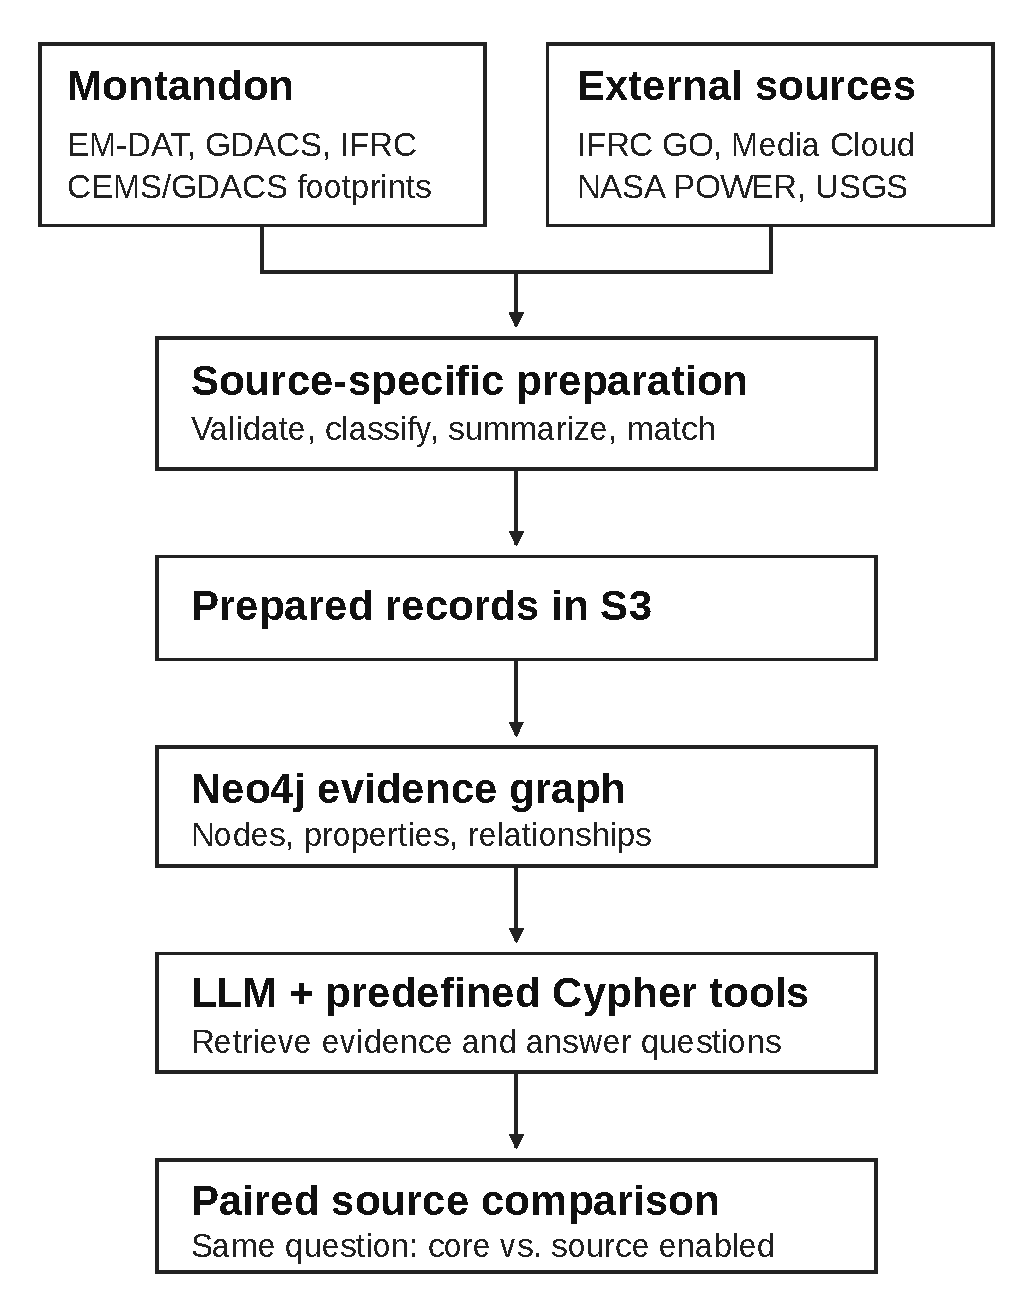
\includegraphics[width=\columnwidth]{fig/figure1_overview.pdf}
    \caption{System workflow from Montandon and external sources to
    graph-based answers and paired source comparison.}
    \label{fig:pipeline}
\end{figure}

\subsection{Neo4j Graph Model}

Montandon records are represented as \texttt{MontandonItem} nodes and
receive \texttt{Event} or \texttt{Impact} labels according to their
record roles. An \texttt{IMPACT\_OF} relationship connects impacts to
events with the same correlation identifier. Events are linked to
country, hazard, and start-date nodes. Description, keyword, and
impact-related embeddings support bounded semantic-similarity
relationships between distinct Montandon records.

IFRC GO events and appeals are represented as \texttt{GOEvent} and
\texttt{GOAppeal} nodes. GO events connect to country nodes, while
\texttt{FOR\_EVENT} links each appeal to the GO event identified in
its source record. A shared country node provides geographic context;
it does not establish that a GO event and a Montandon event are the
same disaster.

Fig.~\ref{fig:graph} distinguishes graph relationships from the
identifier match used to attach weather properties.

\begin{figure}[!t]
    \centering
    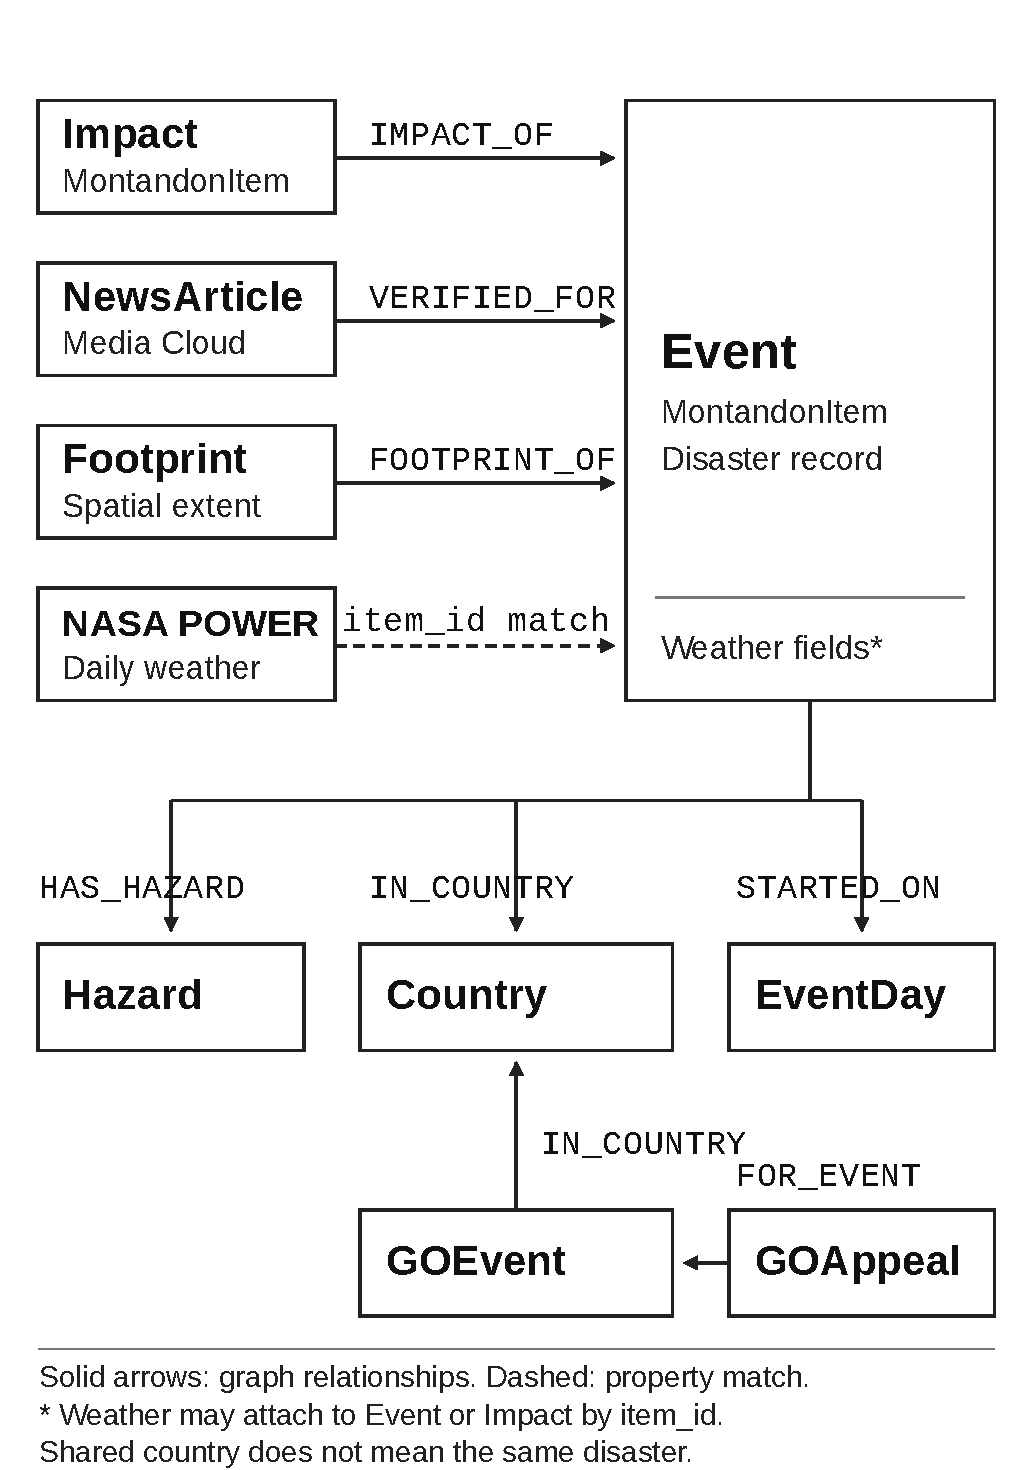
\includegraphics[width=\columnwidth]{fig/figure2_network.pdf}
    \caption{Graph links around a disaster event. Solid arrows are
    relationships; the dashed arrow indicates the identifier match
    used for weather properties.}
    \label{fig:graph}
\end{figure}

\subsection{Connecting Sources to Disaster Records}

The sources require different linkage procedures. News articles do
not share a Montandon event identifier. The news pipeline therefore
compares each candidate with a target event using location, timing,
hazard, and reported effects. An article classified as covering the
same event becomes a \texttt{NewsArticle} node linked to the target
\texttt{Event} by \texttt{VERIFIED\_FOR}. This relationship records an
event-relevance decision; it does not validate every factual claim
in the article.

Weather summaries are attached to the existing
\texttt{MontandonItem} whose identifier matches the collected
weather result's \texttt{item\_id}. Weather is represented as node
properties rather than a separate weather node.

Footprints are linked to \texttt{Event} nodes using matching
correlation identifiers and \texttt{FOOTPRINT\_OF} relationships.
The graph stores footprint summaries and source URLs rather than
full GeoJSON geometry. Retrieved event context distinguishes
Montandon-origin footprints from external USGS ShakeMap footprints.

\subsection{Evidence Retrieval and Answer Generation}

A language-model assistant selects from predefined graph-query tools
for disaster-event searches, event-context retrieval, related-event
searches, IFRC GO response and appeal searches, and news retrieval.
Tool arguments are validated before a predefined Cypher query is
executed. The assistant uses the returned records to compose an
answer and may make further calls within a configured call budget.

Weather summaries and footprint information are returned with
disaster context when available. News articles are retrieved through
a separate \texttt{get\_event\_news} tool. This tool returns saved
articles linked to a selected event, including metadata and article
excerpts. The assistant is instructed to retrieve relevant missing
evidence before concluding that it is unavailable, but tool
selection remains model-driven. Consequently, evaluation records
the tool calls and returned evidence as well as the final answer.

\section{Evaluation Design}

\subsection{EAP-Related Questions}

Evaluation contexts are defined by country and hazard. Five fixed
question templates are instantiated for each selected context:
(1) hazard context and timing, (2) affected areas and vulnerable
groups, (3) responding organizations and coordination, (4) past
actions and needs relevant to early-action choices, and (5) appeal
funding and people targeted. These questions concern historical
evidence that may inform EAP development.

\subsection{Paired Source Comparisons}

For each question, the system first generates a core answer with
news, NASA POWER weather, and external ShakeMap footprints disabled.
The core condition retains Montandon records, Montandon-origin
footprints, and access to IFRC GO tools. The same core answer is
compared separately with an answer generated after enabling one
selected external source: news, weather, or external ShakeMap
footprints.

Source access is controlled at the tool or returned-evidence level.
Disabling news removes the news-retrieval tool. Disabling weather
removes weather fields and weather-based search filters. Disabling
external footprints removes the external-footprint fields while
preserving Montandon-origin footprints. Comparisons therefore
measure the effect of making a source available within this
question-answering workflow. Tool-call records are examined to
determine which evidence the assistant actually retrieved.

\subsection{Contribution Categories}

A judge compares the two answers, their retrieved evidence, and
the question. The rubric assigns one of seven categories:
\texttt{fills\_field} when external evidence supplies a requested
value missing from an existing core field;
\texttt{extends\_coverage} when it answers a requested aspect
outside the core fields; \texttt{qualifies} when it materially
corrects or limits an existing answer; \texttt{corroborates} when it
supports an existing answer without changing it;
\texttt{core\_sufficient} when core evidence already answers the
question; \texttt{unresolved} when requested information remains
missing; and \texttt{unsupported} when an important new or changed
claim is not supported by retrieved evidence.

The rubric checks for unsupported claims first. Additional detail
counts as an improvement only when it addresses the question and is
supported by relevant evidence. For each source and question type,
the improvement rate is the number of evaluated comparisons labeled
\texttt{fills\_field}, \texttt{extends\_coverage}, or
\texttt{qualifies}, divided by the number of evaluated comparisons.
Answer and judgment failures are recorded separately.

\section{Experimental Setup}

% Add the final run's dataset snapshot, selection dates, country--hazard
% contexts, question counts, sources, models, settings, and run metadata.

\section{Results}

% Add the final evaluation results and the corresponding figures here.
% Report attempted and evaluated comparisons separately.

\section{Discussion}

% Interpret source contributions by question type using the final
% results and representative retrieved evidence.

\section{Conclusion}

% Add the main findings and their implications after the final results
% and discussion are established.

\bibliographystyle{IEEEtran}
\bibliography{references}

\end{document}

